\documentclass[12pt]{article}

%packages
%\usepackage{latexsym}
\usepackage{graphicx}
\usepackage{color}
\usepackage{amsmath}
\usepackage{dsfont}
\usepackage{placeins}
\usepackage{amssymb}
\usepackage{wasysym}
\usepackage{abstract}
\usepackage{hyperref}
\usepackage{etoolbox}
\usepackage{datetime}
\usepackage{xcolor}
\usepackage{alphalph}
\settimeformat{ampmtime}

%\usepackage{pstricks,pst-node,pst-tree}

%\usepackage{algpseudocode}
%\usepackage{amsthm}
%\usepackage{hyperref}
%\usepackage{mathrsfs}
%\usepackage{amsfonts}
%\usepackage{bbding}
%\usepackage{listings}
%\usepackage{appendix}
\usepackage[margin=1in]{geometry}
%\geometry{papersize={8.5in,11in},total={6.5in,9in}}
%\usepackage{cancel}
%\usepackage{algorithmic, algorithm}

\makeatletter
\def\maxwidth{ %
  \ifdim\Gin@nat@width>\linewidth
    \linewidth
  \else
    \Gin@nat@width
  \fi
}
\makeatother

\definecolor{fgcolor}{rgb}{0.345, 0.345, 0.345}
\newcommand{\hlnum}[1]{\textcolor[rgb]{0.686,0.059,0.569}{#1}}%
\newcommand{\hlstr}[1]{\textcolor[rgb]{0.192,0.494,0.8}{#1}}%
\newcommand{\hlcom}[1]{\textcolor[rgb]{0.678,0.584,0.686}{\textit{#1}}}%
\newcommand{\hlopt}[1]{\textcolor[rgb]{0,0,0}{#1}}%
\newcommand{\hlstd}[1]{\textcolor[rgb]{0.345,0.345,0.345}{#1}}%
\newcommand{\hlkwa}[1]{\textcolor[rgb]{0.161,0.373,0.58}{\textbf{#1}}}%
\newcommand{\hlkwb}[1]{\textcolor[rgb]{0.69,0.353,0.396}{#1}}%
\newcommand{\hlkwc}[1]{\textcolor[rgb]{0.333,0.667,0.333}{#1}}%
\newcommand{\hlkwd}[1]{\textcolor[rgb]{0.737,0.353,0.396}{\textbf{#1}}}%

\usepackage{framed}
\makeatletter
\newenvironment{kframe}{%
 \def\at@end@of@kframe{}%
 \ifinner\ifhmode%
  \def\at@end@of@kframe{\end{minipage}}%
  \begin{minipage}{\columnwidth}%
 \fi\fi%
 \def\FrameCommand##1{\hskip\@totalleftmargin \hskip-\fboxsep
 \colorbox{shadecolor}{##1}\hskip-\fboxsep
     % There is no \\@totalrightmargin, so:
     \hskip-\linewidth \hskip-\@totalleftmargin \hskip\columnwidth}%
 \MakeFramed {\advance\hsize-\width
   \@totalleftmargin\z@ \linewidth\hsize
   \@setminipage}}%
 {\par\unskip\endMakeFramed%
 \at@end@of@kframe}
\makeatother

\definecolor{shadecolor}{rgb}{.77, .77, .77}
\definecolor{messagecolor}{rgb}{0, 0, 0}
\definecolor{warningcolor}{rgb}{1, 0, 1}
\definecolor{errorcolor}{rgb}{1, 0, 0}
\newenvironment{knitrout}{}{} % an empty environment to be redefined in TeX

\usepackage{alltt}
\usepackage[T1]{fontenc}

\newcommand{\qu}[1]{``#1''}
\newcounter{probnum}
\setcounter{probnum}{1}

%create definition to allow local margin changes
\def\changemargin#1#2{\list{}{\rightmargin#2\leftmargin#1}\item[]}
\let\endchangemargin=\endlist 

%allow equations to span multiple pages
\allowdisplaybreaks

%define colors and color typesetting conveniences
\definecolor{gray}{rgb}{0.5,0.5,0.5}
\definecolor{black}{rgb}{0,0,0}
\definecolor{white}{rgb}{1,1,1}
\definecolor{blue}{rgb}{0.5,0.5,1}
\newcommand{\inblue}[1]{\color{blue}#1 \color{black}}
\definecolor{green}{rgb}{0.133,0.545,0.133}
\newcommand{\ingreen}[1]{\color{green}#1 \color{black}}
\definecolor{yellow}{rgb}{1,1,0}
\newcommand{\inyellow}[1]{\color{yellow}#1 \color{black}}
\definecolor{orange}{rgb}{0.9,0.649,0}
\newcommand{\inorange}[1]{\color{orange}#1 \color{black}}
\definecolor{red}{rgb}{1,0.133,0.133}
\newcommand{\inred}[1]{\color{red}#1 \color{black}}
\definecolor{purple}{rgb}{0.58,0,0.827}
\newcommand{\inpurple}[1]{\color{purple}#1 \color{black}}
\definecolor{backgcode}{rgb}{0.97,0.97,0.8}
\definecolor{Brown}{cmyk}{0,0.81,1,0.60}
\definecolor{OliveGreen}{cmyk}{0.64,0,0.95,0.40}
\definecolor{CadetBlue}{cmyk}{0.62,0.57,0.23,0}

%define new math operators
\DeclareMathOperator*{\argmax}{arg\,max~}
\DeclareMathOperator*{\argmin}{arg\,min~}
\DeclareMathOperator*{\argsup}{arg\,sup~}
\DeclareMathOperator*{\arginf}{arg\,inf~}
\DeclareMathOperator*{\convolution}{\text{\Huge{$\ast$}}}
\newcommand{\infconv}[2]{\convolution^\infty_{#1 = 1} #2}
%true functions

%%%% GENERAL SHORTCUTS

%shortcuts for pure typesetting conveniences
\newcommand{\bv}[1]{\boldsymbol{#1}}

%shortcuts for compound constants
\newcommand{\BetaDistrConst}{\dfrac{\Gamma(\alpha + \beta)}{\Gamma(\alpha)\Gamma(\beta)}}
\newcommand{\NormDistrConst}{\dfrac{1}{\sqrt{2\pi\sigma^2}}}

%shortcuts for conventional symbols
\newcommand{\tsq}{\tau^2}
\newcommand{\tsqh}{\hat{\tau}^2}
\newcommand{\sigsq}{\sigma^2}
\newcommand{\sigsqsq}{\parens{\sigma^2}^2}
\newcommand{\sigsqovern}{\dfrac{\sigsq}{n}}
\newcommand{\tausq}{\tau^2}
\newcommand{\tausqalpha}{\tau^2_\alpha}
\newcommand{\tausqbeta}{\tau^2_\beta}
\newcommand{\tausqsigma}{\tau^2_\sigma}
\newcommand{\betasq}{\beta^2}
\newcommand{\sigsqvec}{\bv{\sigma}^2}
\newcommand{\sigsqhat}{\hat{\sigma}^2}
\newcommand{\sigsqhatmlebayes}{\sigsqhat_{\text{Bayes, MLE}}}
\newcommand{\sigsqhatmle}[1]{\sigsqhat_{#1, \text{MLE}}}
\newcommand{\bSigma}{\bv{\Sigma}}
\newcommand{\bSigmainv}{\bSigma^{-1}}
\newcommand{\thetavec}{\bv{\theta}}
\newcommand{\thetahat}{\hat{\theta}}
\newcommand{\thetahatmle}{\hat{\theta}_{\mathrm{MLE}}}
\newcommand{\thetavechatmle}{\hat{\thetavec}_{\mathrm{MLE}}}
\newcommand{\muhat}{\hat{\mu}}
\newcommand{\musq}{\mu^2}
\newcommand{\muvec}{\bv{\mu}}
\newcommand{\muhatmle}{\muhat_{\text{MLE}}}
\newcommand{\lambdahat}{\hat{\lambda}}
\newcommand{\lambdahatmle}{\lambdahat_{\text{MLE}}}
\newcommand{\etavec}{\bv{\eta}}
\newcommand{\alphavec}{\bv{\alpha}}
\newcommand{\minimaxdec}{\delta^*_{\mathrm{mm}}}
\newcommand{\ybar}{\bar{y}}
\newcommand{\xbar}{\bar{x}}
\newcommand{\Xbar}{\bar{X}}
\newcommand{\phat}{\hat{p}}
\newcommand{\Phat}{\hat{P}}
\newcommand{\Zbar}{\bar{Z}}
\newcommand{\iid}{~{\buildrel iid \over \sim}~}
\newcommand{\inddist}{~{\buildrel ind \over \sim}~}
\newcommand{\approxdist}{~{\buildrel approx \over \sim}~}
\newcommand{\equalsindist}{~{\buildrel d \over =}~}
\newcommand{\loglik}[1]{\ell\parens{#1}}
\newcommand{\thetahatkminone}{\thetahat^{(k-1)}}
\newcommand{\thetahatkplusone}{\thetahat^{(k+1)}}
\newcommand{\thetahatk}{\thetahat^{(k)}}
\newcommand{\half}{\frac{1}{2}}
\newcommand{\third}{\frac{1}{3}}
\newcommand{\twothirds}{\frac{2}{3}}
\newcommand{\fourth}{\frac{1}{4}}
\newcommand{\fifth}{\frac{1}{5}}
\newcommand{\sixth}{\frac{1}{6}}

%shortcuts for vector and matrix notation
\newcommand{\A}{\bv{A}}
\newcommand{\At}{\A^T}
\newcommand{\Ainv}{\inverse{\A}}
\newcommand{\B}{\bv{B}}
\newcommand{\K}{\bv{K}}
\newcommand{\Kt}{\K^T}
\newcommand{\Kinv}{\inverse{K}}
\newcommand{\Kinvt}{(\Kinv)^T}
\newcommand{\M}{\bv{M}}
\newcommand{\Bt}{\B^T}
\newcommand{\Q}{\bv{Q}}
\newcommand{\Qt}{\Q^T}
\newcommand{\R}{\bv{R}}
\newcommand{\Rt}{\R^T}
\newcommand{\Z}{\bv{Z}}
\newcommand{\X}{\bv{X}}
\newcommand{\Xsub}{\X_{\text{(sub)}}}
\newcommand{\Xsubadj}{\X_{\text{(sub,adj)}}}
\newcommand{\I}{\bv{I}}
\newcommand{\Y}{\bv{Y}}
\newcommand{\sigsqI}{\sigsq\I}
\renewcommand{\P}{\bv{P}}
\newcommand{\Psub}{\P_{\text{(sub)}}}
\newcommand{\Pt}{\P^T}
\newcommand{\Pii}{P_{ii}}
\newcommand{\Pij}{P_{ij}}
\newcommand{\IminP}{(\I-\P)}
\newcommand{\Xt}{\bv{X}^T}
\newcommand{\XtX}{\Xt\X}
\newcommand{\XtXinv}{\parens{\Xt\X}^{-1}}
\newcommand{\XtXinvXt}{\XtXinv\Xt}
\newcommand{\XXtXinvXt}{\X\XtXinvXt}
\newcommand{\x}{\bv{x}}
\newcommand{\onevec}{\bv{1}}
\newcommand{\oneton}{1, \ldots, n}
\newcommand{\yoneton}{y_1, \ldots, y_n}
\newcommand{\yonetonorder}{y_{(1)}, \ldots, y_{(n)}}
\newcommand{\Yoneton}{Y_1, \ldots, Y_n}
\newcommand{\iinoneton}{i \in \braces{\oneton}}
\newcommand{\onetom}{1, \ldots, m}
\newcommand{\jinonetom}{j \in \braces{\onetom}}
\newcommand{\xoneton}{x_1, \ldots, x_n}
\newcommand{\Xoneton}{X_1, \ldots, X_n}
\newcommand{\xt}{\x^T}
\newcommand{\y}{\bv{y}}
\newcommand{\yt}{\y^T}
\renewcommand{\c}{\bv{c}}
\newcommand{\ct}{\c^T}
\newcommand{\tstar}{\bv{t}^*}
\renewcommand{\u}{\bv{u}}
\renewcommand{\v}{\bv{v}}
\renewcommand{\a}{\bv{a}}
\newcommand{\s}{\bv{s}}
\newcommand{\yadj}{\y_{\text{(adj)}}}
\newcommand{\xjadj}{\x_{j\text{(adj)}}}
\newcommand{\xjadjM}{\x_{j \perp M}}
\newcommand{\yhat}{\hat{\y}}
\newcommand{\yhatsub}{\yhat_{\text{(sub)}}}
\newcommand{\yhatstar}{\yhat^*}
\newcommand{\yhatstarnew}{\yhatstar_{\text{new}}}
\newcommand{\z}{\bv{z}}
\newcommand{\zt}{\z^T}
\newcommand{\bb}{\bv{b}}
\newcommand{\bbt}{\bb^T}
\newcommand{\bbeta}{\bv{\beta}}
\newcommand{\beps}{\bv{\epsilon}}
\newcommand{\bepst}{\beps^T}
\newcommand{\e}{\bv{e}}
\newcommand{\Mofy}{\M(\y)}
\newcommand{\KofAlpha}{K(\alpha)}
\newcommand{\ellset}{\mathcal{L}}
\newcommand{\oneminalph}{1-\alpha}
\newcommand{\SSE}{\text{SSE}}
\newcommand{\SSEsub}{\text{SSE}_{\text{(sub)}}}
\newcommand{\MSE}{\text{MSE}}
\newcommand{\RMSE}{\text{RMSE}}
\newcommand{\SSR}{\text{SSR}}
\newcommand{\SST}{\text{SST}}
\newcommand{\JSest}{\delta_{\text{JS}}(\x)}
\newcommand{\Bayesest}{\delta_{\text{Bayes}}(\x)}
\newcommand{\EmpBayesest}{\delta_{\text{EmpBayes}}(\x)}
\newcommand{\BLUPest}{\delta_{\text{BLUP}}}
\newcommand{\MLEest}[1]{\hat{#1}_{\text{MLE}}}

%shortcuts for Linear Algebra stuff (i.e. vectors and matrices)
\newcommand{\twovec}[2]{\bracks{\begin{array}{c} #1 \\ #2 \end{array}}}
\newcommand{\threevec}[3]{\bracks{\begin{array}{c} #1 \\ #2 \\ #3 \end{array}}}
\newcommand{\fivevec}[5]{\bracks{\begin{array}{c} #1 \\ #2 \\ #3 \\ #4 \\ #5 \end{array}}}
\newcommand{\twobytwomat}[4]{\bracks{\begin{array}{cc} #1 & #2 \\ #3 & #4 \end{array}}}
\newcommand{\threebytwomat}[6]{\bracks{\begin{array}{cc} #1 & #2 \\ #3 & #4 \\ #5 & #6 \end{array}}}

%shortcuts for conventional compound symbols
\newcommand{\thetainthetas}{\theta \in \Theta}
\newcommand{\reals}{\mathbb{R}}
\newcommand{\complexes}{\mathbb{C}}
\newcommand{\rationals}{\mathbb{Q}}
\newcommand{\integers}{\mathbb{Z}}
\newcommand{\naturals}{\mathbb{N}}
\newcommand{\forallninN}{~~\forall n \in \naturals}
\newcommand{\forallxinN}[1]{~~\forall #1 \in \reals}
\newcommand{\matrixdims}[2]{\in \reals^{\,#1 \times #2}}
\newcommand{\inRn}[1]{\in \reals^{\,#1}}
\newcommand{\mathimplies}{\quad\Rightarrow\quad}
\newcommand{\mathlogicequiv}{\quad\Leftrightarrow\quad}
\newcommand{\eqncomment}[1]{\quad \text{(#1)}}
\newcommand{\limitn}{\lim_{n \rightarrow \infty}}
\newcommand{\limitN}{\lim_{N \rightarrow \infty}}
\newcommand{\limitd}{\lim_{d \rightarrow \infty}}
\newcommand{\limitt}{\lim_{t \rightarrow \infty}}
\newcommand{\limitsupn}{\limsup_{n \rightarrow \infty}~}
\newcommand{\limitinfn}{\liminf_{n \rightarrow \infty}~}
\newcommand{\limitk}{\lim_{k \rightarrow \infty}}
\newcommand{\limsupn}{\limsup_{n \rightarrow \infty}}
\newcommand{\limsupk}{\limsup_{k \rightarrow \infty}}
\newcommand{\floor}[1]{\left\lfloor #1 \right\rfloor}
\newcommand{\ceil}[1]{\left\lceil #1 \right\rceil}

%shortcuts for environments
\newcommand{\beqn}{\vspace{-0.25cm}\begin{eqnarray*}}
\newcommand{\eeqn}{\end{eqnarray*}}
\newcommand{\bneqn}{\vspace{-0.25cm}\begin{eqnarray}}
\newcommand{\eneqn}{\end{eqnarray}}

%shortcuts for mini environments
\newcommand{\parens}[1]{\left(#1\right)}
\newcommand{\squared}[1]{\parens{#1}^2}
\newcommand{\tothepow}[2]{\parens{#1}^{#2}}
\newcommand{\prob}[1]{\mathbb{P}\parens{#1}}
\newcommand{\cprob}[2]{\prob{#1~|~#2}}
\newcommand{\littleo}[1]{o\parens{#1}}
\newcommand{\bigo}[1]{O\parens{#1}}
\newcommand{\Lp}[1]{\mathbb{L}^{#1}}
\renewcommand{\arcsin}[1]{\text{arcsin}\parens{#1}}
\newcommand{\prodonen}[2]{\bracks{\prod_{#1=1}^n #2}}
\newcommand{\mysum}[4]{\sum_{#1=#2}^{#3} #4}
\newcommand{\sumonen}[2]{\sum_{#1=1}^n #2}
\newcommand{\infsum}[2]{\sum_{#1=1}^\infty #2}
\newcommand{\infprod}[2]{\prod_{#1=1}^\infty #2}
\newcommand{\infunion}[2]{\bigcup_{#1=1}^\infty #2}
\newcommand{\infinter}[2]{\bigcap_{#1=1}^\infty #2}
\newcommand{\infintegral}[2]{\int^\infty_{-\infty} #2 ~\text{d}#1}
\newcommand{\supthetas}[1]{\sup_{\thetainthetas}\braces{#1}}
\newcommand{\bracks}[1]{\left[#1\right]}
\newcommand{\braces}[1]{\left\{#1\right\}}
\newcommand{\set}[1]{\left\{#1\right\}}
\newcommand{\abss}[1]{\left|#1\right|}
\newcommand{\norm}[1]{\left|\left|#1\right|\right|}
\newcommand{\normsq}[1]{\norm{#1}^2}
\newcommand{\inverse}[1]{\parens{#1}^{-1}}
\newcommand{\rowof}[2]{\parens{#1}_{#2\cdot}}

%shortcuts for functionals
\newcommand{\realcomp}[1]{\text{Re}\bracks{#1}}
\newcommand{\imagcomp}[1]{\text{Im}\bracks{#1}}
\newcommand{\range}[1]{\text{range}\bracks{#1}}
\newcommand{\colsp}[1]{\text{colsp}\bracks{#1}}
\newcommand{\rowsp}[1]{\text{rowsp}\bracks{#1}}
\newcommand{\tr}[1]{\text{tr}\bracks{#1}}
\newcommand{\rank}[1]{\text{rank}\bracks{#1}}
\newcommand{\proj}[2]{\text{Proj}_{#1}\bracks{#2}}
\newcommand{\projcolspX}[1]{\text{Proj}_{\colsp{\X}}\bracks{#1}}
\newcommand{\median}[1]{\text{median}\bracks{#1}}
\newcommand{\mean}[1]{\text{mean}\bracks{#1}}
\newcommand{\dime}[1]{\text{dim}\bracks{#1}}
\renewcommand{\det}[1]{\text{det}\bracks{#1}}
\newcommand{\expe}[1]{\mathbb{E}\bracks{#1}}
\newcommand{\expeabs}[1]{\expe{\abss{#1}}}
\newcommand{\expesub}[2]{\mathbb{E}_{#1}\bracks{#2}}
\newcommand{\indic}[1]{\mathds{1}_{#1}}
\newcommand{\var}[1]{\mathbb{V}\text{ar}\bracks{#1}}
\newcommand{\cov}[2]{\mathbb{C}\text{ov}\bracks{#1, #2}}
\newcommand{\corr}[2]{\text{Corr}\bracks{#1, #2}}
\newcommand{\se}[1]{\mathbb{S}\text{E}\bracks{#1}}
\newcommand{\seest}[1]{\hat{\mathbb{S}\text{E}}\bracks{#1}}
\newcommand{\bias}[1]{\text{Bias}\bracks{#1}}
\newcommand{\derivop}[2]{\dfrac{\text{d}}{\text{d} #1}\bracks{#2}}
\newcommand{\partialop}[2]{\dfrac{\partial}{\partial #1}\bracks{#2}}
\newcommand{\secpartialop}[2]{\dfrac{\partial^2}{\partial #1^2}\bracks{#2}}
\newcommand{\mixpartialop}[3]{\dfrac{\partial^2}{\partial #1 \partial #2}\bracks{#3}}

%shortcuts for functions
\renewcommand{\exp}[1]{\mathrm{exp}\parens{#1}}
\renewcommand{\cos}[1]{\text{cos}\parens{#1}}
\renewcommand{\sin}[1]{\text{sin}\parens{#1}}
\newcommand{\sign}[1]{\text{sign}\parens{#1}}
\newcommand{\are}[1]{\mathrm{ARE}\parens{#1}}
\newcommand{\natlog}[1]{\ln\parens{#1}}
\newcommand{\oneover}[1]{\frac{1}{#1}}
\newcommand{\overtwo}[1]{\frac{#1}{2}}
\newcommand{\overn}[1]{\frac{#1}{n}}
\newcommand{\oneoversqrt}[1]{\oneover{\sqrt{#1}}}
\newcommand{\sqd}[1]{\parens{#1}^2}
\newcommand{\loss}[1]{\ell\parens{\theta, #1}}
\newcommand{\losstwo}[2]{\ell\parens{#1, #2}}
\newcommand{\cf}{\phi(t)}

%English language specific shortcuts
\newcommand{\ie}{\textit{i.e.} }
\newcommand{\AKA}{\textit{AKA} }
\renewcommand{\iff}{\textit{iff}}
\newcommand{\eg}{\textit{e.g.} }
\newcommand{\st}{\textit{s.t.} }
\newcommand{\wrt}{\textit{w.r.t.} }
\newcommand{\mathst}{~~\text{\st}~~}
\newcommand{\mathand}{~~\text{and}~~}
\newcommand{\ala}{\textit{a la} }
\newcommand{\ppp}{posterior predictive p-value}
\newcommand{\dd}{dataset-to-dataset}

%shortcuts for distribution titles
\newcommand{\logistic}[2]{\mathrm{Logistic}\parens{#1,\,#2}}
\newcommand{\bernoulli}[1]{\mathrm{Bernoulli}\parens{#1}}
\newcommand{\betanot}[2]{\mathrm{Beta}\parens{#1,\,#2}}
\newcommand{\stdbetanot}{\betanot{\alpha}{\beta}}
\newcommand{\multnormnot}[3]{\mathcal{N}_{#1}\parens{#2,\,#3}}
\newcommand{\normnot}[2]{\mathcal{N}\parens{#1,\,#2}}
\newcommand{\classicnormnot}{\normnot{\mu}{\sigsq}}
\newcommand{\stdnormnot}{\normnot{0}{1}}
\newcommand{\uniformdiscrete}[1]{\mathrm{Uniform}\parens{\braces{#1}}}
\newcommand{\uniform}[2]{\mathrm{U}\parens{#1,\,#2}}
\newcommand{\stduniform}{\uniform{0}{1}}
\newcommand{\geometric}[1]{\mathrm{Geometric}\parens{#1}}
\newcommand{\hypergeometric}[3]{\mathrm{Hypergeometric}\parens{#1,\,#2,\,#3}}
\newcommand{\exponential}[1]{\mathrm{Exp}\parens{#1}}
\newcommand{\gammadist}[2]{\mathrm{Gamma}\parens{#1, #2}}
\newcommand{\poisson}[1]{\mathrm{Poisson}\parens{#1}}
\newcommand{\binomial}[2]{\mathrm{Binomial}\parens{#1,\,#2}}
\newcommand{\negbin}[2]{\mathrm{NegBin}\parens{#1,\,#2}}
\newcommand{\rayleigh}[1]{\mathrm{Rayleigh}\parens{#1}}
\newcommand{\multinomial}[2]{\mathrm{Multinomial}\parens{#1,\,#2}}
\newcommand{\gammanot}[2]{\mathrm{Gamma}\parens{#1,\,#2}}
\newcommand{\cauchynot}[2]{\text{Cauchy}\parens{#1,\,#2}}
\newcommand{\invchisqnot}[1]{\text{Inv}\chisq{#1}}
\newcommand{\invscaledchisqnot}[2]{\text{ScaledInv}\ncchisq{#1}{#2}}
\newcommand{\invgammanot}[2]{\text{InvGamma}\parens{#1,\,#2}}
\newcommand{\chisq}[1]{\chi^2_{#1}}
\newcommand{\ncchisq}[2]{\chi^2_{#1}\parens{#2}}
\newcommand{\ncF}[3]{F_{#1,#2}\parens{#3}}

%shortcuts for PDF's of common distributions
\newcommand{\logisticpdf}[3]{\oneover{#3}\dfrac{\exp{-\dfrac{#1 - #2}{#3}}}{\parens{1+\exp{-\dfrac{#1 - #2}{#3}}}^2}}
\newcommand{\betapdf}[3]{\dfrac{\Gamma(#2 + #3)}{\Gamma(#2)\Gamma(#3)}#1^{#2-1} (1-#1)^{#3-1}}
\newcommand{\normpdf}[3]{\frac{1}{\sqrt{2\pi#3}}\exp{-\frac{1}{2#3}(#1 - #2)^2}}
\newcommand{\normpdfvarone}[2]{\dfrac{1}{\sqrt{2\pi}}e^{-\half(#1 - #2)^2}}
\newcommand{\chisqpdf}[2]{\dfrac{1}{2^{#2/2}\Gamma(#2/2)}\; {#1}^{#2/2-1} e^{-#1/2}}
\newcommand{\invchisqpdf}[2]{\dfrac{2^{-\overtwo{#1}}}{\Gamma(#2/2)}\,{#1}^{-\overtwo{#2}-1}  e^{-\oneover{2 #1}}}
\newcommand{\exponentialpdf}[2]{#2\exp{-#2#1}}
\newcommand{\poissonpdf}[2]{\dfrac{e^{-#1} #1^{#2}}{#2!}}
\newcommand{\binomialpdf}[3]{\binom{#2}{#1}#3^{#1}(1-#3)^{#2-#1}}
\newcommand{\rayleighpdf}[2]{\dfrac{#1}{#2^2}\exp{-\dfrac{#1^2}{2 #2^2}}}
\newcommand{\gammapdf}[3]{\dfrac{#3^#2}{\Gamma\parens{#2}}#1^{#2-1}\exp{-#3 #1}}
\newcommand{\cauchypdf}[3]{\oneover{\pi} \dfrac{#3}{\parens{#1-#2}^2 + #3^2}}
\newcommand{\Gammaf}[1]{\Gamma\parens{#1}}

%shortcuts for miscellaneous typesetting conveniences
\newcommand{\notesref}[1]{\marginpar{\color{gray}\tt #1\color{black}}}

%%%% DOMAIN-SPECIFIC SHORTCUTS

%Real analysis related shortcuts
\newcommand{\zeroonecl}{\bracks{0,1}}
\newcommand{\forallepsgrzero}{\forall \epsilon > 0~~}
\newcommand{\lessthaneps}{< \epsilon}
\newcommand{\fraccomp}[1]{\text{frac}\bracks{#1}}

%Bayesian related shortcuts
\newcommand{\yrep}{y^{\text{rep}}}
\newcommand{\yrepisq}{(\yrep_i)^2}
\newcommand{\yrepvec}{\bv{y}^{\text{rep}}}


%Probability shortcuts
\newcommand{\SigField}{\mathcal{F}}
\newcommand{\ProbMap}{\mathcal{P}}
\newcommand{\probtrinity}{\parens{\Omega, \SigField, \ProbMap}}
\newcommand{\convp}{~{\buildrel p \over \rightarrow}~}
\newcommand{\convLp}[1]{~{\buildrel \Lp{#1} \over \rightarrow}~}
\newcommand{\nconvp}{~{\buildrel p \over \nrightarrow}~}
\newcommand{\convae}{~{\buildrel a.e. \over \longrightarrow}~}
\newcommand{\convau}{~{\buildrel a.u. \over \longrightarrow}~}
\newcommand{\nconvau}{~{\buildrel a.u. \over \nrightarrow}~}
\newcommand{\nconvae}{~{\buildrel a.e. \over \nrightarrow}~}
\newcommand{\convd}{~{\buildrel \mathcal{D} \over \rightarrow}~}
\newcommand{\nconvd}{~{\buildrel \mathcal{D} \over \nrightarrow}~}
\newcommand{\withprob}{~~\text{w.p.}~~}
\newcommand{\io}{~~\text{i.o.}}

\newcommand{\Acl}{\bar{A}}
\newcommand{\ENcl}{\bar{E}_N}
\newcommand{\diam}[1]{\text{diam}\parens{#1}}

\newcommand{\taua}{\tau_a}

\newcommand{\myint}[4]{\int_{#2}^{#3} #4 \,\text{d}#1}
\newcommand{\laplacet}[1]{\mathscr{L}\bracks{#1}}
\newcommand{\laplaceinvt}[1]{\mathscr{L}^{-1}\bracks{#1}}
\renewcommand{\min}[1]{\text{min}\braces{#1}}
\renewcommand{\max}[1]{\text{max}\braces{#1}}

\newcommand{\Vbar}[1]{\bar{V}\parens{#1}}
\newcommand{\expnegrtau}{\exp{-r\tau}}

%%% problem typesetting
\definecolor{darkgrey}{rgb}{0.10,0.10,0.9}

\newcommand{\problem}[1]{\noindent \colorbox{black}{{\color{yellow} \large{\textsf{\textbf{Problem \arabic{probnum}}}}~}} \addtocounter{probnum}{1} \vspace{0.2cm} \\ \iftoggle{professormode}{}{\color{darkgrey}} #1}

\newcommand{\easysubproblem}[1]{\ingreen{\item} \iftoggle{professormode}{}{\color{darkgrey}} [easy] #1 \color{black} }
\newcommand{\intermediatesubproblem}[1]{\inorange{\item} \iftoggle{professormode}{}{\color{darkgrey}} [harder] #1 \color{black} }
\newcommand{\hardsubproblem}[1]{\inred{\item} \iftoggle{professormode}{}{\color{darkgrey}} [difficult] #1 \color{black} }
\newcommand{\extracreditsubproblem}[1]{\inpurple{\item} \iftoggle{professormode}{}{\color{darkgrey}} [E.C.] #1 \color{black} }


\newcommand{\spc}[1]{\iftoggle{professormode}{\\ \vspace{#1cm}}{\\ \vspace{-0.3cm}}}

\makeatletter
\newalphalph{\alphmult}[mult]{\@alph}{26}
\renewcommand{\labelenumi}{(\alphmult{\value{enumi}})}

\newcommand{\support}[1]{\text{Supp}\bracks{#1}}
\newcommand{\mode}[1]{\text{Mode}\bracks{#1}}
\newcommand{\IQR}[1]{\text{IQR}\bracks{#1}}
\newcommand{\quantile}[2]{\text{Quantile}\bracks{#1,\,#2}}

\newtoggle{professormode}
\toggletrue{professormode} %STUDENTS: DELETE or COMMENT this line



\title{MATH 342W / 650.4 / RM742 Spring \the\year~HW \#1}

\author{Loyd Flores} %STUDENTS: write your name here

\iftoggle{professormode}{
\date{Due 11:59PM February 11, \the\year~by email \\ \vspace{0.5cm} \small (this document last updated \currenttime~on \today)}
}

\renewcommand{\abstractname}{Instructions and Philosophy}

\begin{document}
\maketitle

\iftoggle{professormode}{
\begin{abstract}
The path to success in this class is to do many problems. Unlike other courses, exclusively doing reading(s) will not help. Coming to lecture is akin to watching workout videos; thinking about and solving problems on your own is the actual ``working out.''  Feel free to \qu{work out} with others; \textbf{I want you to work on this in groups.}

Reading is still \textit{required}. For this homework set, read the first chapter of \qu{Learning from Data} and the introduction and Chapter 1 of Silver's book. Of course, you should be googling and reading about all the concepts introduced in class online. This is your responsibility to supplement in-class with your own readings.

The problems below are color coded: \ingreen{green} problems are considered \textit{easy} and marked \qu{[easy]}; \inorange{yellow} problems are considered \textit{intermediate} and marked \qu{[harder]}, \inred{red} problems are considered \textit{difficult} and marked \qu{[difficult]} and \inpurple{purple} problems are extra credit. The \textit{easy} problems are intended to be ``giveaways'' if you went to class. Do as much as you can of the others; I expect you to at least attempt the \textit{difficult} problems. 

This homework is worth 100 points but the point distribution will not be determined until after the due date. See syllabus for the policy on late homework.

Up to 7 points are given as a bonus if the homework is typed using \LaTeX. Links to instaling \LaTeX~and program for compiling \LaTeX~is found on the syllabus. You are encouraged to use \url{overleaf.com}. If you are handing in homework this way, read the comments in the code; there are two lines to comment out and you should replace my name with yours and write your section. The easiest way to use overleaf is to copy the raw text from hwxx.tex and preamble.tex into two new overleaf tex files with the same name. If you are asked to make drawings, you can take a picture of your handwritten drawing and insert them as figures or leave space using the \qu{$\backslash$vspace} command and draw them in after printing or attach them stapled.

The document is available with spaces for you to write your answers. If not using \LaTeX, print this document and write in your answers. I do not accept homeworks which are \textit{not} on this printout. Keep this first page printed for your records.

\end{abstract}

\thispagestyle{empty}
\vspace{1cm}
NAME: Loyd Flores
\clearpage
}

\problem{These are questions about Silver's book, the introduction and chapter 1.}

\begin{enumerate}

\easysubproblem{What is the difference between \emph{predict} and \emph{forecast}? Are these two terms used interchangeably today?} \\ \\
\textbf{Answer:} \\
As Seraydarian defines, "Prediction involves estimating an outcome with a high level of certainty, usually based on historical data and statistical modeling. On the other hand, a forecast involves projecting future developments but with a certain level of uncertainty due to external factors that may impact the outcome." This helps us understand how Silver defines prediction. It is "what the soothsayer told you." Soothsayer being the data that tells us the story on how we can make predictions. Forecast on the other hand is defined as "implied planning under conditions of uncertainty. It suggested having prudence, wisdom, and industriousness." Which aligns with Cassius' idea that a man is a master of his own fate as forecasting utilizes the user's foresight to a greater extent. Although these differences are clearly defined, in contemporary usage, the two terms are often used interchangeably, a point also noted in Silver's book.

\vspace{10pt}
\noindent
Citation: Seraydarian, L. (2023, August 11). Prediction vs forecasting. Plat.AI. Retrieved from \url{https://plat.ai/blog/difference-between-prediction-and-forecast/} \\

\easysubproblem{What is John P. Ioannidis's findings and what are its implications?} \\

\textbf{Answer:} \\
John P. Ioannidis released a paper titled “Why Most Published Research Findings Are False.” Bayer Laboratories confirmed John's findings, as they were unable to replicate about two-thirds of the positive findings claimed in medical journals when they attempted the experiments themselves. In my interpretation, John's findings imply that the experiments in these published journals may have had controlled variables which could not be replicated. We can conclude that the findings were false due to the irreproducible nature of these findings, which means they are not true in all cases or when other external variables are introduced. \\ 


\easysubproblem{What are the human being's most powerful defense (according to Silver)? Answer using the language from class.} \\ \\
\textbf{Answer:} \\ 
Silver asserts that our most potent defense lies in our wits. Human minds are more agile than those of any other species, uniquely equipped to discern patterns and rapidly respond to both opportunities and threats. This aligns with our class discussions, where we emphasized humans' capacity to learn and recognize patterns through data analysis. Furthermore, humans excel in assessing situations, as displayed by Jefferson's quote, "Early to bed, early to rise makes a man healthy, wealthy, and wise." This proverb presents our ability to evaluate and improve our circumstances proactively. In the modern era, we have even extended this capability through technology, developing methodologies like machine learning to process and interpret data at unprecedented rates, thereby augmenting our inherent strengths. \\


% Continue with more content or questions...



\easysubproblem{Information is increasing at a rapid pace, but what is not increasing?} \\ \\
\textbf{Answer:} \\ 
Since the development of the printing press in the 1400s, there has been a rapid increase in the production of information, as evidenced by the proliferation of books and other forms of consumable text. This acceleration is also reflected in the timeline of human development: it took 300 years to transition into the industrial age, but only 200 years after that for the internet to become a dominant force in our lives. The technological advancement gap is narrowing further, with AI emerging just 20 years after the internet's inception. However, as Silver notes in his book, what is not keeping pace with this rapid increase of information is the human capacity to process and digest it. The surge in data availability means there is also a corresponding rise in false or misleading information, creating a challenge for humans who must now sift through this vast expanse of data without adequate time for proper analysis and understanding. \\
\hardsubproblem{Silver admits that we will always be subjectively biased when making predictions. However, he believes there is an objective truth. In class, how did we describe the objective truth? Answer using notation from class i.e. $t,f, g, h^*, \delta, \epsilon, t, z_1, \ldots, z_t, \delta, \mathbb{D}$, $\mathcal{H}, \mathcal{A}, \mathcal{X}, \mathcal{Y}, X, y, n, p$, $x_{\cdot 1}, \ldots, x_{\cdot p}, , \ldots, x_{n \cdot}$, etc.} \\ \\ \\

\textbf{Answer:} \\ In class, we discussed the concept of 'objective truth,' denoted as `f`. It is the closest approximation we have to `y`, which are real world results, and ideally fits our data. However, the objective truth, or `f`, is unattainable due to its complexity. The closest we can get to `f` is with `h*`, a function within `H`, our set of functions or hypothesis set, which has the lowest error. The function `h` is selected by `A`, our learning algorithm. With everything previously stated, we can develop `g`, our model that takes `x` (which could be values from `X`, our input space) to produce an approximation of `y`. The model `g` is formulated by inputting `D`, our data or a sample of our data, and `H` into `A`. This process produces the best combination of these components to come up with our model, `g`. \\ \\

\easysubproblem{In a nutshell, what is Karl Popper's (a famous philosopher of science) definition of \emph{science}?} \\

\textbf{Answer:}\\
For Karl Popper a philosopher of science states that science is composed of hypothesis that could be tested in the real world by means of prediction. In a nutshell if we are unable to test a hypothesis in the real world then it is not scientific. \\

\intermediatesubproblem{Why did the ratings agencies say the probability of a CDO defaulting was 0.12\% instead of the 28\% that actually occured? Answer using concepts from class.} \\

\textbf{Answer:}\\
Referencing concepts from our class the rating agencies predicted only .12\% due to the availability of their data or in our lectures terms `D`. Their model was based off of previous events and they failed to account for what ended up happening. The error they had was really due to ignorance because the data they needed was not available. One can argue that they could've based off of the housing market crash in Japan that happened which was in recent history during those times. \\

\easysubproblem{What is the difference between \emph{risk} and \emph{uncertainty} according to Silver's definitions?}\\

\textbf{Answer:} \\
Silver defines `risk` as something we can quantify or put a price on. We understand the likelihood of such risks occurring and the potential effects if we experience the consequences of those risks. On the other hand, `uncertainty` refers to risks that are difficult to measure. With uncertainty, one can never fully comprehend the entire context. The best one can achieve is a vague understanding of the situation, but never a complete picture. \\ 
\hardsubproblem{How does Silver define \emph{out of sample}? Answer using notation from class i.e. $t,f, g, h^*, \delta, \epsilon, z_1, \ldots, z_t, \delta, \mathbb{D}, \mathcal{H}, \mathcal{A}, \mathcal{X}, \mathcal{Y}, X, y, n, p, x_{\cdot 1}, \ldots, x_{\cdot p}, x_{1 \cdot}, \ldots, x_{n \cdot}$, etc. WARNING: Silver defines \emph{out of sample} completely differently than the literature, than practitioners in industry and how we will define it in class in a month or so. We will explore what he is talking about in class in the future and we will term this concept differently, using the more widely accepted terminology. So please forget the phrase \emph{out of sample} for now as we will introduce it later in class as something else. There will be other such terms in his book and I will provide this disclaimer at these appropriate times.} \\ \\
\textbf{Answer: } \\
Silver defines out of sample as something that had never been seen before. He gave the example of the rapid increase in U.S. housing that proceeded the collapse. In our lectures context there were data points `x` that were not in `X`, our input space. The model that we have was only familiar with data points in our `D` and was performing well because it had very low `error`. The problem is a point `x` that was out of sample and the model was only able to predict based on the available data in `D` making the prediction wrong because of a large error due to  ignorance. 

\\

\intermediatesubproblem{Look up \emph{bias} and \emph{variance} online or in a statistics textbook. Connect these concepts to Silver's terms \emph{accuracy} and \emph{precision}. This is another example of Silver using non-standard terminology.}\\

\textbf{Answer:} \\ 

In a statistical context, bias is the error that occurs when we approximate a real-world problem in simplified terms, despite its complexity. Bias measures how far off a model's predictions are from the actual value. High bias may indicate that a model is oversimplified and fails to consider all variables or relationships. Variance, on the other hand, is defined as the model's sensitivity to fluctuations or noise in the dataset. It measures how predictions for a point might vary between different realizations of the model or the extent of the spread between predictions. A model with high variance is so complex that it captures even the noise within the data patterns, performing well with training data but failing with unseen data. Connecting this to Silver's definitions: bias relates to the accuracy of the model, meaning that if the model makes errors, it will consistently do so in the same direction. It may result in our model consistently hitting the same spot, but not the target. Variance is related to precision. As previously defined, variance is the spread of the data; in Silver's terms, it addresses how far off our shots are. Low precision equates to high variance. If our shots are all close together, we have high precision or low variance. This can mislead the engineer because high precision does not necessarily equate to quality. \\
Citation: \\
Bias (Statistics) (2024/02/10). In Wikipedia. \url{https://en.wikipedia.org/wiki/Bias\_(statistics)} \\ 

Hayes, A. (2023, December 19). \textit{What Is Variance in Statistics? Definition, Formula, and Example}. Retrieved from: \url{https://www.investopedia.com/terms/v/variance.asp}
\end{enumerate}


\problem{Below are some questions about the theory of modeling.}

\begin{enumerate}

\easysubproblem{Redraw the illustration of Earth and the table-top globe except do not use the Earth and a table-top globe as examples (use another example). The quadrants are connected with arrows. Label these arrows appropriately.}\\
\textbf{Image : }\\
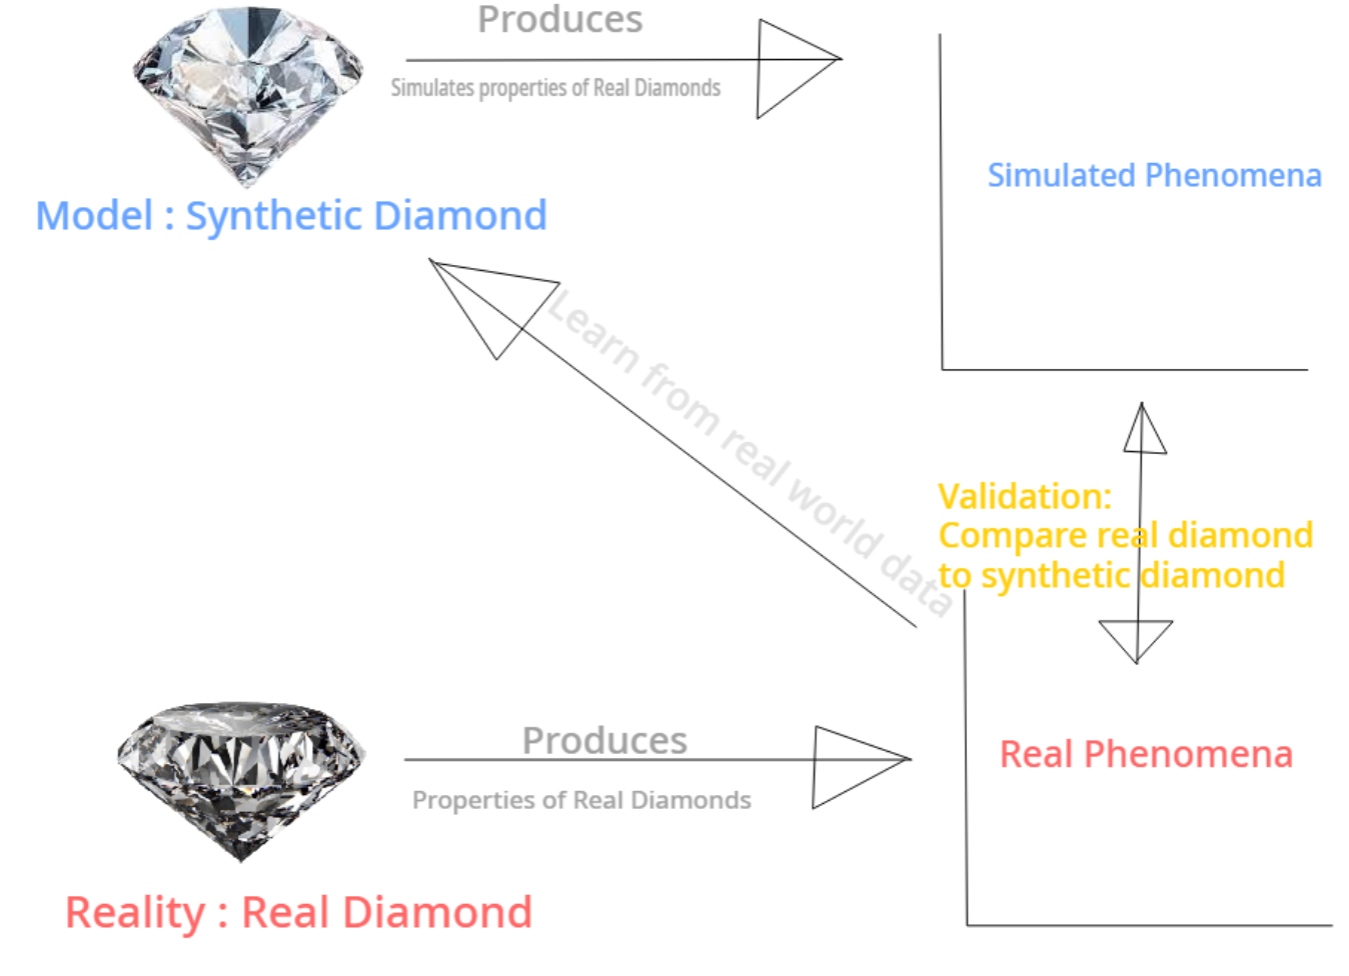
\includegraphics[width=\linewidth]{model-drawing.png} \\

\easysubproblem{Pursuant to the fix in the previous question, how do we define \emph{data} for the purposes of this class?}\\

\textbf{Answer: } \\
Pursuant to the previous question data is defined to be the properties of something real. Referring to the previous example it could be the size, weight, hardness, and other properties of a diamond that could produce real phenomena as such as how it is created or how it could withstand immense pressure. In the context of our class the diamonds' properties could be our `D`
\\


\easysubproblem{Pursuant to the fix in the previous question, how do we define \emph{predictions} for the purposes of this class?}\\

\textbf{Answer: } \\
Pursuant to the previous question prediction in our class is defined as the actualization of our hypothesis on the available data that we have. Using the illustration presented the prediction is a synthetic diamond. We cam up with this conclusion using real properties of a diamond. Calculations are made to simulate the diamond which could be our `h`. We can then validate our synthetic diamond to the real one by comparing their properties. 
\\

\easysubproblem{Why are \qu{all models wrong}? We are quoting the famous statisticians George Box and Norman Draper here.}\\

\textbf{Answer: } \\ 
George Box says "All models are wrong but some could be useful". This is true because a model is just an approximation of reality. Models will never be the real thing. Some models are useful because it can help us navigate reality but as previously stated can never be the absolute truth. \\ 

\intermediatesubproblem{Why are \qu{[some models] useful}? We are quoting the famous statisticians George Box and Norman Draper here.}\\
Some models are useful because they are really fine tuned. They can produce really close results to reality sometimes the difference can be so minute you can assume it is reality, keyword `assume`. Models are still models meaning they are only approximations and we can only assume. It is not the absolute truth therefore it can be useful to guide us. 
\\

\intermediatesubproblem{What is the difference between a "good model" and a "bad model"?}\\ 
\textbf{Answer: } \\ 
In my understanding a good model accurately predicts the outcome desired and generalizes well to unseen data while a bad model fails to make accurate predictions beyond the data it was trained on, sometimes failing to even make accurate predictions on training data. \\
\end{enumerate}




\problem{We are now going to investigate the famous English aphorism \qu{an apple a day keeps the doctor away} as a model. We will use this as springboard to ask more questions about the framework of modeling we introduced in this class.}

\begin{enumerate}


\easysubproblem{Is this a mathematical model? Yes / no and why.}\\
\textbf{Answer: } \\
In my opinion It is not a mathematical model. It is merely a proverb. A mathematical model is a little more complex than a proverb. There has to be a quantifiable relationship. Also I don't see what kind of equation we can produce out of this. Although if I had to make this a mathematical model, I could attempt to learn the relationship of consumed apples to number of doctor visits both in an annual time frame.

\easysubproblem{What is(are) the input(s) in this model?}\\
\textbf{Answer: } \\ 
The inputs for this could be the following `x1`: \# of apples consumed daily, `x2`: \# of annual doctor's visits. We could optionally add other measures of health such as the amount of times you caught a cold or got sick, etc ...
\easysubproblem{What is(are) the output(s) in this model?}\\
\textbf{Answer: }\\ 
The output of our model could either predict the number of visits annually, instead of it being an input it could be our output. We could also produce a model that would accept x being the number of apples consumed and it would determine whether or not it will reduce your \# of visits or if it improved via a binary response y/n where it would learn through data collected. \\ 
\\

\intermediatesubproblem{How good / bad do you think this model is and why?}\\
\textbf{Answer: } \\ 
I think this model will be bad. It would be as good as a random person predicting this. I don't think there is a correlation because yes an apple is nutritious but it isn't the sole determinant to whether or not it can keep you away from the doctor. There are other factors on why you would visit the doctor that is not health related. I don't see an empirical solution to this problem just by the number of apples consumed.
\\

\easysubproblem{Devise a metric for gauging the main input. Call this $x_1$ going forward.}\\
\textbf{Answer: } \\
As I previously stated above `x1` could be the total number of apples consumed annually or it could be average apples consumed per month. The consumption rate could be scaled up or down depending on how the Data scientist will prefer their units.\\

\easysubproblem{Devise a metric for gauging the main output. Call this $y$ going forward.}\\
\textbf{Answer :} \\
`y` could possibly a binary classification of y/n that determines if you visit a doctor in a specific time frame, or if your medical bills increased or decreased given a time frame. It could also become a regression model where it tries to predict medical bills or total number of medical visits. \\

\easysubproblem{What is $\mathcal{Y}$ mathematically?}\\
\textbf{Answer: } \\ 
$\mathcal{Y}$ = g(x), where g is our model and `x` in `X` which is our input space. \\ 

\easysubproblem{Briefly describe $z_1, \ldots, z_t$ in English where $y = t(z_1, \ldots, z_t)$ in this \emph{phenomenon} (not \emph{model}).}\\ 
\textbf{Answer: } \\ 
`z`'s are what contribute to our prediction `y`. `z`'s could be a wide array of things that could potentially affect our result. In this phenomenon the `z`'s could be the number of apples consumed for example. This could affect whether or not we go to the doctor or how much we spend on the doctor.

\easysubproblem{From this point on, you only observe $x_1$. What is the value of $p$?}\\ 
\textbf{Answer: } \\ 
I defined my `x1` to be average number of apples consumed in a month. With that being said this in itself will not predict p or even contribute that's why I could say that p = .5. We have a 50-50 chance to getting it wrong because its no better than a random guess. \\ 


\intermediatesubproblem{What is $\mathcal{X}$ mathematically? If your information contained in $x_1$ is non-numeric, you must coerce it to be numeric at this point.}\\ 
\textbf{Answer: }\\
$X = \{ x \in \mathbb{R} \mid x \geq 0 \}$ We give this formula to make x quantifiable. The least we can have is 0, we cant have a negative consumption of apples.

\easysubproblem{How did we term the functional relationship between $y$ and $x_1$? Is it approximate or equals?}\\
\textbf{Answer: } \\ 
$y \approx f(x)$  We can only approximate y and it will never be equals. \\ 


\easysubproblem{Briefly describe \emph{superivised learning}.}\\
\textbf{Answer: } \\ 
Supervised learning is when we have a target label available in our data. We can use this target label to verify our predictions to see whether we are right or wrong. This is where the term supervised comes from because we are using the target to guide us. 

\easysubproblem{Why is \emph{superivised learning} an \emph{empirical solution} and not an \emph{analytic solution}?}\\ 
\textbf{Answer: } \\ 
Supervised learning is considered to be empirical because it is built solely on available data. It is data driven in a sense that it needs targeted data sets to be considered a supervised learning model. It will be great to have theoretical background but it requires the data more than anything else hence an empirical solution. \\ 

\intermediatesubproblem{From this point on, assume we are involved in supervised learning to achieve the goal you stated in the previous question. Briefly describe what $\mathbb{D}$ would look like here.}\\
\textbf{Answer: }
 $\mathbb{D}$ = <X1...Xn, Yn>. X1...Xn would be the column or features and it would range from 1 to n which would be the number of columns. Y would be the result or the prediction obtained using the available data.
\intermediatesubproblem{Briefly describe the role of $\mathcal{H}$ and $\mathcal{A}$ here.}\spc{5} \\ 
\textbf{Answer: } \\ 
In the framework of machine learning, \( \mathcal{H} \) represents the hypothesis space, which is the set of all possible functions or models that could be used to fit our data \( D \). This space encompasses every conceivable model.

On the other hand, \( \mathcal{A} \) is the learning algorithm. Its role is to search through the hypothesis space \( \mathcal{H} \) to find the most suitable model that effectively captures the relationship inherent in the data \( D \). The algorithm does this by evaluating different models within \( \mathcal{H} \) based on their performance, often using a criterion such as minimizing error.

\easysubproblem{If $g = \mathcal{A}(\mathbb{D}, \mathcal{H})$, what should the domain and range of $g$ be?} \\ 
\textbf{Answer: } \\ 
The domain of this problem will be all possible input pairs in $\mathbb{D}$ evaluated by all possible `h`'s in $ \mathcal{H}$. The range will be the dot product of the two or all possible outcomes from all the configurations of data points and evaluating functions.

\easysubproblem{Is $g \in \mathcal{H}$? Why or why not?} \\
\textbf{Answer: } \\ 
$g \in \mathcal{H}$ because $\mathcal{A}$ selects the best performing h in $\mathcal{H}$. The g we end up with performed the best by attaining lowest error in the set of all available functions. 

\easysubproblem{Given a never-before-seen value of $x_1$ which we denote $x^*$, what formula would we use to predict the corresponding value of the output? Denote this prediction $\hat{y}^*$.} \\
\textbf{Answer: } \\ 
$\hat{y}^*$ = g($x^*$). Where the unseen data is taken by our model to spit out a prediction.

\intermediatesubproblem{$f$ is the function that is the best possible fit of the phenomenon given the covariates. We will unfortunately not be able to define \qu{best} until later in the course. But you can think of it as a device that extracts all possible information from the covariates and whatever is left over $\delta$ is due exclusively to information you do not have. Is it reasonable to assume $f \in \mathcal{H}$? Why or why not?}\\
\textbf{Answer: } \\
It is highly unlikely that f is in H because f perfectly fits to our data. f is something that we are trying to attain. If anything f maybe too complex to even exist due to its perfect nature. H is the set of available functions that we have sometimes it is over simplistic by being only linear models.  \\ 

\easysubproblem{In the general modeling setup, if $f \notin \mathcal{H}$, what are the three sources of error? Copy the equation from the class notes. Denote the names of each error and provide a sentence explanation of each. Denote also $e$ and $\mathcal{E}$ using underbraces / overbraces.}\\
\textbf{Answer: } \\
The entire equation is as follows 
y = $g(x_1, \ldots, x_p) + (h^*(x_1, \ldots, x_p) - g(x_1, \ldots, x_p)) + (f(x_1, \ldots, x_p) - h^*(x_1, \ldots, x_p)) + \delta$. Where $g(x_1, \ldots, x_p)$ is our model. Estimation error is basically when our model is unable to capture the relationship of our data points this could occur because either we have too few data or there is too much noise in the data we have. It is denoted by $`(h^*(x_1, \ldots, x_p) - g(x_1, \ldots, x_p))`$, we can reduce estimation error by collecting more data so g converges to H*. The next error is specification error which is caused by our model oversimplifying the relationships in our data we can solve this by utilizing more complex models. It is denoted by `$(f(x_1, \ldots, x_p) - h^*(x_1, \ldots, x_p))$`. The last type of error is delta which is denoted by `$\delta$` or could referred to as Ignorance error. This is basically the error alloted because we don't really know or have data about certain things, the best we have are proxies. 


\easysubproblem{In the general modeling setup, for each of the three source of error, explain what you would do to reduce the source of error as best as you can.}\\
\textbf{Answer: }\\ 
Estimation error could be reduced by adding more data. With more data our model will be more capable of identifying relationships between variables. Mis-specification error is caused by our model being unable to unable to fit to our data maybe because it is too complex. This is solved by utilizing more complex functions that will be able to fit with the data. The last error is error due to ignorance which is the hardest one to compensate. The only way I can think of is by collecting domain-specific data or having an expert on the team to add more analytical judgement. \\ 


\intermediatesubproblem{In the general modeling setup, make up an $f$, an $h^*$ and a $g$ and plot them on a graph of $y$ vs $x$ (assume $p=1$). Indicate the sources of error on this plot (see last question). Which source of error is missing from the picture? Why?}\\
\textbf{Image: }
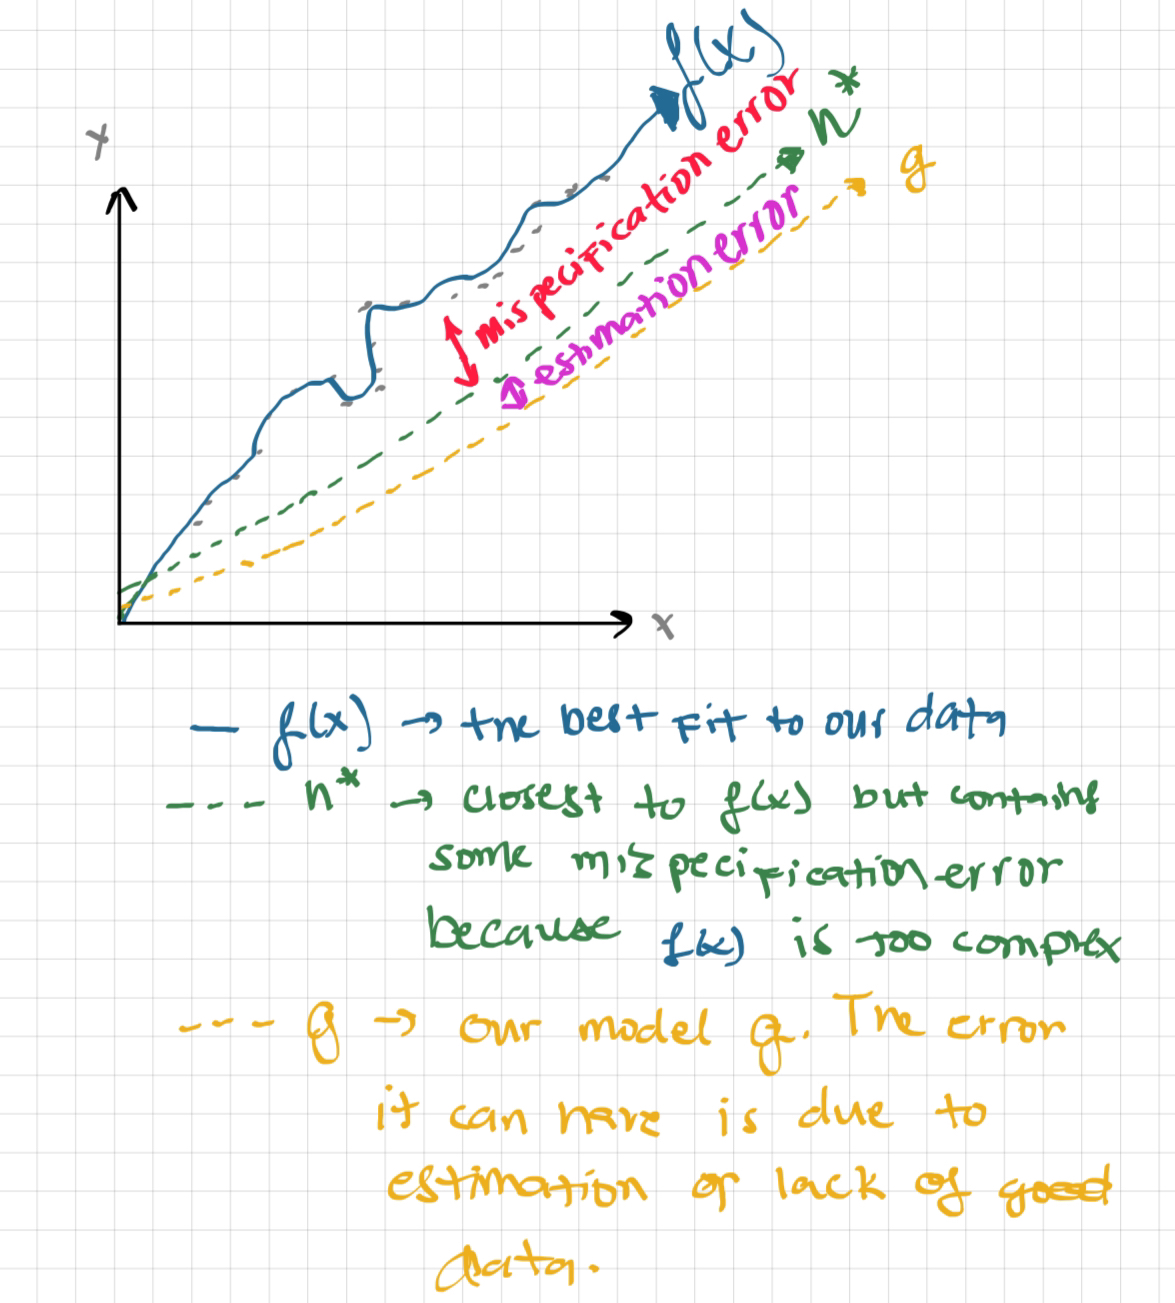
\includegraphics[width=\linewidth]{math342w-3.v.png} \\

\easysubproblem{What is a null model $g_0$? What data does it make use of? What data does it not make use of?}\\
\textbf{Answer: } \\
$g_0$ or the null model is a baseline model only taking into consideration y and none of the other features in X. The purpose of this model is to benchmark the performance of other models that could be more complex. If a model fails to outperform the null model it means that said model is unable to capture the relationship in our data or the engineer probably did something wrong in the process. \\ 


\easysubproblem{What is a parameter in $\mathcal{H}$?}\\
\textbf{Author: } \\ 
In my understanding a parameter is a value that defines a particular model within the space. each h in H could be characterized by a set of parameters which determines how a model behaves and fits data. For a regression model it could be the intercept of a line. Intercepts could define how h will interact with the data. For complex models like neural networks parameters could be weights of different variables which would be adjusted throught iterations.

Citation: n/a (2024, February 11). "Hypothesis Parameters in Machine Learning". Retrieved from \url{https://chat.openai.com/c/dedf1ec2-b14d-4eac-8729-0f0bd4863f0c} (ChatGPT)\\

\easysubproblem{Regardless of your answer to what $\mathcal{Y}$ was above in (g), we now coerce $\mathcal{Y} = \braces{0,1}$. What would the null model $g_0$ be and why?}\\
\textbf{Answer: } \\ 

The null model $g_0$ is a baseline model that only considers  $y$. It will predict the most frequent occurrence of a class in $y$. The accuracy then becomes the percentage of the appearance of that most frequently occurring class in our dataset.

\easysubproblem{Regardless of your answer to what $\mathcal{Y}$ was above in (g), we now coerce $\mathcal{Y} = \braces{0,1}$. If we use a threshold model, what would $\mathcal{H}$ be? What would the parameter(s) be?}\\
\textbf{Answer: } \\ 
$\mathcal{H}$ would consist of all functions that could produce a binary output.The parameters in this context would be the threshold. Each h in $\mathcal{H}$ could have different set threshold as they will all interact with the data differently. In summary $\mathcal{H}$ will consist of different ways we can combine data and the parameter would be the threshold which would be how they each method of combination would handle data differently. 

\easysubproblem{Give an explicit example of $g$ under the threshold model.}\\
\textbf{Answer: } \\ 
For example g = 2x+3 and our threshold is 5. Our model  takes x as input and will spit out a binary classification of yes/no. If g(x) > 5, then the output is yes. Else g(x) < 5, the output is no.

\end{enumerate}


\problem{As alluded to in class, modeling is synonymous with the entire enterprise of science. 

In 1964, \href{https://en.wikipedia.org/wiki/Richard_Feynman}{Richard Feynman}, a famous physicist and public intellectual with an inimitably captivating presentation style, gave a series of seven lectures in 1964 at Cornell University on the \qu{character of physical law}. Here is a \href{https://www.youtube.com/watch?v=EYPapE-3FRw}{10min excerpt} of one of these lectures about the scientific method. Feel free to watch the entire clip, but for the purposes of this class, we are only interested in the following segments: 0:00-1:00 and 3:48-6:45. }

\begin{enumerate}


\intermediatesubproblem{According to Feynman, how does the scientific method differ from learning from data with regards to building models for reality? (0:08)} \\ 
\textbf{Answer: } \\ 
Feynman discusses that the scientific method involves. First we guess it, then we compute the consequences of the guess to see what it implies, then we compare the results to nature or experiment. If it disagrees it is wrong. Learning from data approaches this differently by analyzing existing data to find patterns before making any predictions which is opposite to Feynman's scientific method. \\ 


\intermediatesubproblem{He uses the phrase \qu{compute consequences}. What word did we use in class for \qu{compute consequences}? This word also appears in your diagram in 2a. (0:14)}\\
\textbf{Answer: } \\ 
In the context of our lectures we used the term 'Validation' where we compare the phenomena of our simulation or model to the phenomena of real world data. 

\intermediatesubproblem{When he says compare consequences to \qu{experiment}, what word did we use in class for \qu{experiment}? This word also appears in your diagram in 2a. (0:29)}\\
\textbf{Answer:} \\ 
In the context of our class instead of experiment we use prediction or learn from data. The prediction is our experiment based off the patterns we learned by analyzing our data. \\

\intermediatesubproblem{When he says \qu{compare consequences to experiment}, which part of the diagram in 2a is that comparison?}\\ 
\textbf{Answer: } \\
Validation or where we compare our model's phenomena to the real world's phenomena.

\hardsubproblem{When he says \qu{if it disagrees with experiment, it's wrong} (0:44), would a data scientist agree/disagree? What would the data scientist further comment?}\\
\textbf{Answer: } \\ 
Feynman's quote says that if your hypothesis doesn't align with the experiment there is no way around it, your hypothesis is just wrong, plain and simple. A data scientist may argue because the objective function we posses as of now is way to simple. The necessary model maybe more complex. Another concern could be the data, it may just mean we lack data. A data scientist may argue that a process is not just binary right or wrong, there maybe more underlying reasons as to why our model could be wrong now but could be corrected looking forward. \\ 

\hardsubproblem{[You can skip his UFO discussion as it belongs in a class on statistical inference on the topic of $H_0$ vs $H_a$ which is \emph{not} in the curriculum of this class.] He then goes on to say \qu{We can disprove any definite theory. We never prove [a theory] right... We can only be sure we're wrong} (3:48 - 5:08). What does this mean about models in the context of our class?} \\ 
\textbf{Answer: } \\ 
Feynman quotes that we only prove guesses wrong and never right. As long as a theory stand it's not wrong but also is not right, it just stands. This happens due to the lack of knowledge we have in status quo. Something may be understood the way it is now but in the future more complex systems and analyses could exist that could disprove a theory that stands today. In the context of mathematical models it is pretty similar. There are some models that are unable to fit towards data that is present due to its complexity. For example before they only had the Perceptron Algorithm that is able to find the best model that could split the data into 2 sections. Throughout time more complex models were developed and the perceptron is barely used in present day. \\ 

\hardsubproblem{Further he says, \qu{you cannot prove a \emph{vague} theory wrong} (5:10 - 5:48). What does this mean in the context of mathematical models and metrics?} \\
\textbf{Answer: } \\
If a theory is not clear and specific, it's hard to prove it wrong because it doesn't clearly state what it's about. It uses unclear standards that are not measured correctly. There might be parts of the theory that don't really show how they are connected to what you're trying to prove, making you think the theory could be right just because it's not specific enough. Proving such a theory wrong is tough because its vagueness can make it seem right, even if it isn't. It would also be hard to dispprove such vague theory because it will be difficult to test against it due to its vague nature. \\

\hardsubproblem{He then he continues with an example from psychology. Remeber in the 1960's psychoanalysis was very popular. What is his remedy for being able to prove the vague psychology theory right (5:49 - 6:29)?} \\
\textbf{Answer: } \\ 
Feynman states that "It would be possible to state ahead of time if how much is not enough and how much is overindulgent." This means that if we were to quantify the available parameters we have better by having thresholds it would make our hypothesis testable. He says that if we quantify our problem better then an explanation can come out of it. \\ 

\hardsubproblem{He then says \qu{then you can't claim to know anything about it} (6:40). Why can't you know anything about it?} \\
\textbf{Answer: }\\ 
In my interpretation this means that if your hypothesis is vaguely defined or if the variables in the hypothesis is not quantified properly despite whatever answer you get it is not correct. You can't claim to know anything when your hypothesis can't even be tested or proven right or wrong. If you can't even define your problem, you won't be able to answer it. \\ 
\spc{5}

Just to demonstrate that this modeling enterprise is all over science (not just Physics), I present to you the controversial theoretical political scientist John Mearsheimer. He's all over youtube and there's nothing special about this video that I will link here about \href{https://www.youtube.com/watch?v=D_Mx_e8t7nU&t=4673s}{Can China Rise Peacefully?} Feel free to watch the entire clip, but for the purposes of this class, we are only interested in the following segments referenced in the questions which has nothing to do with China, only his theory of \qu{power politics}.

\hardsubproblem{Is Mearsheimer's model of great power politics / international relations (i.e., modern history) 9:35-17:22 simple or complicated? Explain.} \\
\textbf{Answer: } \\ 
John Mearsheimer's model of great power politics is both simple and complicated. It depends on the perspective from which it is viewed.
It could become simple because there is a clear theoretical framework. It is based on five basic assumptions about the nature of international relations, making it straightforward. It is also consistent with realism. He aligns the model will realist perspective. With the previous points mentioned the model then becomes predictable which makes it simple. It can also become complicated because when applied to diverse scenarios adding the complexity of the real world and international relations the model then becomes really complicated. The diversity of states, contexts, history, and etc.. add even more layers of complexity. We also then have to understand the intentions of other states'. This is a problem because we have to sort situations out where everyone wins which most of the time is impossible.  We also have to add inconsideration the natural of power politics. The shifting balance of power makes the context a little more dynamic. Solutions or negotiations that could happen now may not be able to push through tomorrow. In summary the model in itself is simple and straightforward it gets difficult when applying this to the real world where there are a multitude of variables that could change the outcome.  \\ 

\hardsubproblem{Summarize his ideas about limitations of his theory from 39:18-40:00 using vocabulary from this class.} \\
\textbf{Answer: } \\ 
John Mearsheimer states that most theories can never get everything right and all theories have limits because theories are simplification of real world scenarios. He even states that the best models can get things right 75\% of the time and wrong 25\% of the time. In the context of our class models behave in the same way. The best models today are the best of status quo but could be developed as years go by. Our models will always have limitations and can never be the absolute truth mainly because it is only an approximation of reality. Models can also fall short to other things such as oversimplified models that attempt to understand very complex data. There is also a big portion of error that models obtain due to the fact that we don't really know the entire context of the real world. There is just error due to ignorance. As we develop our models like John states we hope to further develop our models more and more as time goes by.

\end{enumerate}

\end{document}

\end{document}

%%%%%%%%%%%%%%%%%This following will go in the next homework!!!



\problem{These are questions about the linear perceptron. This problem is not related to problem 3.}

\begin{enumerate}

\easysubproblem{For the linear perceptron model and the linear support vector machine model, what is $\mathcal{H}$? Use $b$ as the bias term.}\spc{3}

\intermediatesubproblem{Rewrite the steps of the \emph{perceptron learning algorithm} using $b$ as the bias term.}\spc{13}

\easysubproblem{Illustrate the perceptron as a one-layer neural network with the Heaviside / binary step / indicator function activation function.}\spc{10}

\easysubproblem{Provide an illustration of a two-layer neural network. Be careful to indicate all pieces. If a mathematical object has a different value from another mathematical object, denote it differently.}\spc{10}

\end{enumerate}

